\documentclass[a4wide,10pt]{article}
%\usepackage{a4wide}
\usepackage[applemac,utf8]{inputenc}
%\usepackage[danish]{babel}
\usepackage[T1]{fontenc}
\usepackage{pdfsync}
\usepackage{amsmath,amssymb,amsfonts} 
\usepackage[pdftex]{graphicx}
%\usepackage{wrapfig}
%\usepackage{color}
\usepackage[small,bf]{caption}

\begin{document}
\title{DSB Portfolio 2}
\author{Nis Sarup}
\date{\today}
\maketitle

\newpage

	\section{Fourier Transform method} % (fold)
	\label{sec:fourier_transform_method}
		Mathematica functions:
		\begin{eqnarray}
			t &=& 67; \nonumber \\
			m &=& \frac{t-1}{2}; \nonumber \\
			cH &:=& \frac{2\pi 1800}{8000}; \nonumber \\
			cL &:=& \frac{2\pi 800}{8000}; \nonumber \\
			h[0] &:=& \frac{cH-cL}{\pi}; \nonumber \\
			h[n\_] &:=& \frac{Sin[cH \cdot n]}{n\cdot \pi} - \frac{Sin[cL \cdot n]}{n\cdot \pi}; \nonumber \\
		\end{eqnarray}
		I get the results h[n] with n ranging from $-m$ to $m$:
		\begin{equation}
			Table[h[i], {i, -m, m, 1}] \nonumber
		\end{equation}
		This gives a large table of values which I copy into the MathLab program (Program 7.1 for example 7.3 in the book) and get the following graph:
		\begin{figure}[h]
			\centering
				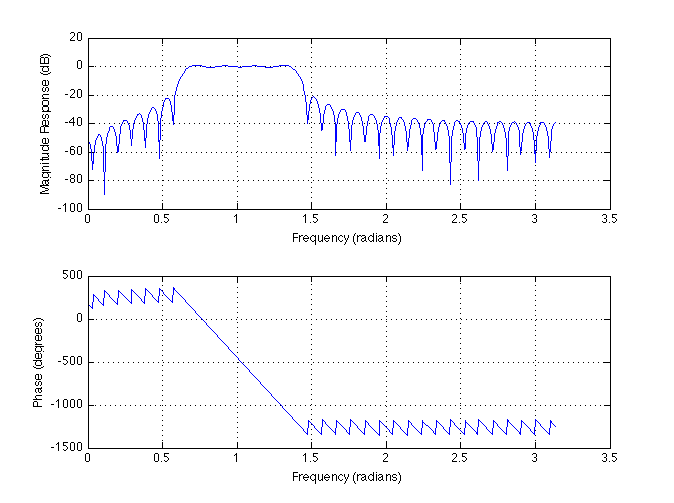
\includegraphics[width=9cm]{images/opgave_1.png}
			\caption{Fourier Transform method: Magnitude response and Phase.}
			\label{fig:images_opgave_1}
		\end{figure}
	% section fourier_transform_method (end)
	
	\newpage
	
	\section{Window Method} % (fold)
	\label{sec:window_method}
		\subsection{Rectangular Window} % (fold)
		\label{sub:rectangular_window}
			Mathematica function for the rectangular window:
			\begin{equation}
				rectangularWindow[n\_] := 1; \nonumber
			\end{equation}
			Not overly exciting. 
			For each value in the set from Section 1 I multiply it with the corresponding value from the window function. Here is a plot of the "new" graphs. 
			\begin{figure}[h]
				\centering
					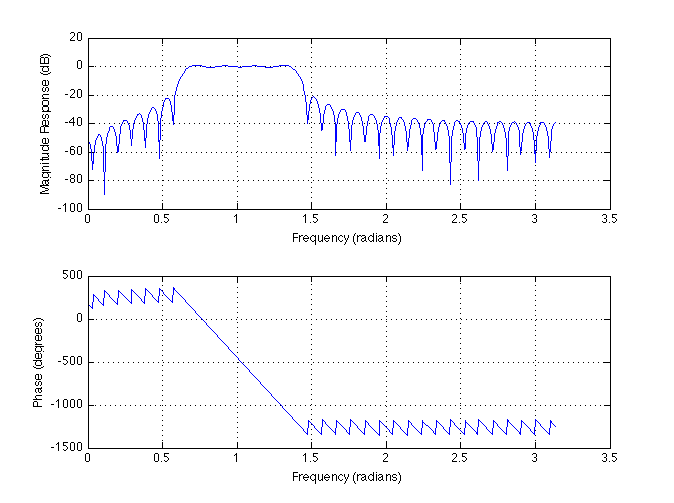
\includegraphics[width=9cm]{images/opgave_2_a.png}
				\caption{Rectangular window: Magnitude response and Phase.}
				\label{fig:images_opgave_2_a}
			\end{figure}
			Not surprisingly both Figure 1 and Figure 2 looks quite similar.
		% subsection rectangular_window (end)
		
\newpage		
		\subsection{Hamming Window} % (fold)
		\label{sub:hamming_window}
			Mathematica function for the Hamming Window:
			\begin{equation}
				hammingWindow[n\_] := 0.54 + 0.46 Cos[\frac{n\cdot \pi}{m}]; \nonumber
			\end{equation}
			Same procedure as with the Rectangular window. As can be seen there are some changes on this graph.
			\begin{figure}[h]
				\centering
					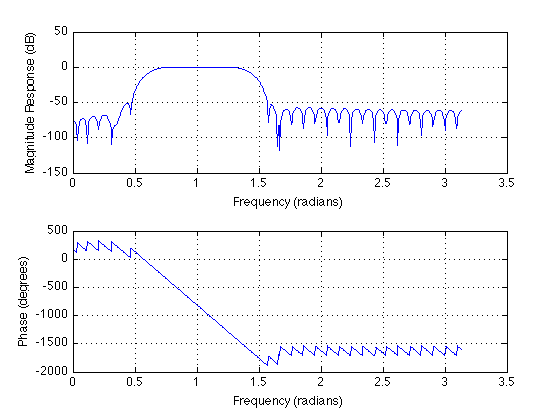
\includegraphics[width=9cm]{images/opgave_2_b.png}
				\caption{Hamming window: Magnitude response and Phase.}
				\label{fig:images_opgave_2_b}
			\end{figure}
			
		% subsection hamming_window (end)
		
\newpage
		\subsection{Kaiser Window} % (fold)
		\label{sub:kaiser_window}
		Mathlab has a build-in Kaiser-function, so I use that to generate the Kaiser window-values:
		\begin{eqnarray}
			beta &=& 0.5842*(50-21)^{0.4}+0.07886*(50-21); \nonumber \\
			wkaiser &=& kaiser(67, beta); \nonumber \\
		\end{eqnarray}
		THat particular equation for the Kaiser window is chosen because the specification calls for a stopband attenuation at 50dB.
		Again the values are multiplied and graphed.
		\begin{figure}[h]
			\centering
				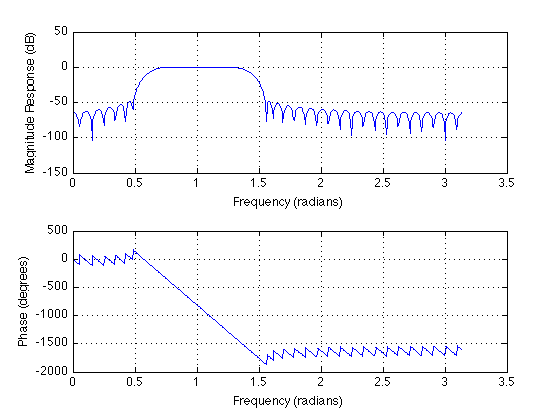
\includegraphics[width=9cm]{images/opgave_2_c.png}
			\caption{Kaiser window: Magnitude response and Phase.}
			\label{fig:images_opgave_2_c}
		\end{figure}
		
		% subsection kaiser_window (end)
	% section window_method (end)
	
\end{document}